\documentclass[11pt,letterpaper]{article}
\usepackage[english]{babel}
\usepackage[utf8]{inputenc}
\usepackage{fancyhdr}
\usepackage[margin=1in]{geometry}
\usepackage{enumitem}
\usepackage{amsmath}
\usepackage{graphicx}
\usepackage{setspace} 
\onehalfspacing
 
\pagestyle{fancy}
\fancyhf{}
\lhead{STAT 423 HW 1}
\rhead{Nan Tang (1662478)}
\rfoot{Page \thepage}
 

\title{STAT 423 Homework 1}
\author{Nan Tang \\ University of Washington}
\date{\today}
 
\begin{document}
\maketitle

\section*{Question 1}
\subsection*{a}
\begin{verbatim}
library(alr4)
age_dt <- sort(unique(wblake$Age))
leng_mean_dt <- numeric(length(age_dt))
for (i in age_dt) {
  leng_mean_dt[i] <- mean(wblake$Length[wblake$Age == i])
}
age_leng_mean_df <- data.frame(age_dt, leng_mean_dt)
plot(age_leng_mean_df, pch=16, ylab='Mean Length', xlab='Age', main='Age vs Mean of Length')
\end{verbatim}

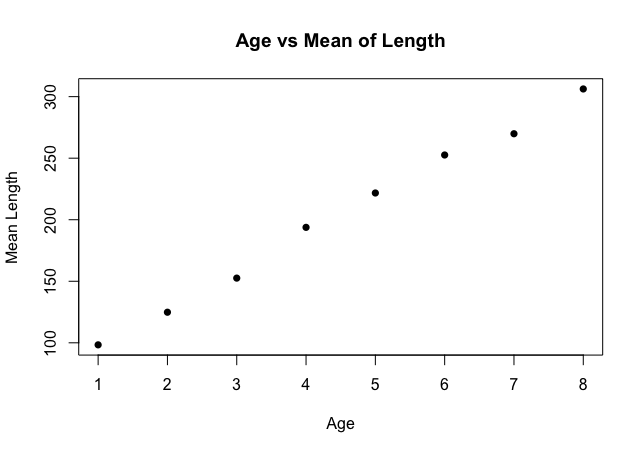
\includegraphics[scale=0.6]{1-a-1.png}

\begin{verbatim}
> age_leng_mean_df
  age_dt leng_mean_dt
1      1     98.34211
2      2    124.84722
3      3    152.56383
4      4    193.80000
5      5    221.72059
6      6    252.59770
7      7    269.86885
8      8    306.25000
\end{verbatim}

\noindent The pattern of scatterplot shows possible linear relation between age and its corresponding mean length.

\subsection*{b}
\begin{verbatim}
leng_sd_dt <- numeric(length(age_dt))
for (i in age_dt) {
  leng_sd_dt[i] <- sd(wblake$Length[wblake$Age == i])
}
age_leng_sd_df <- data.frame(age_dt, leng_sd_dt)
plot(age_leng_sd_df, pch=16, ylab='SD of Length', xlab='Age', main='Age vs SD of Length')
\end{verbatim}

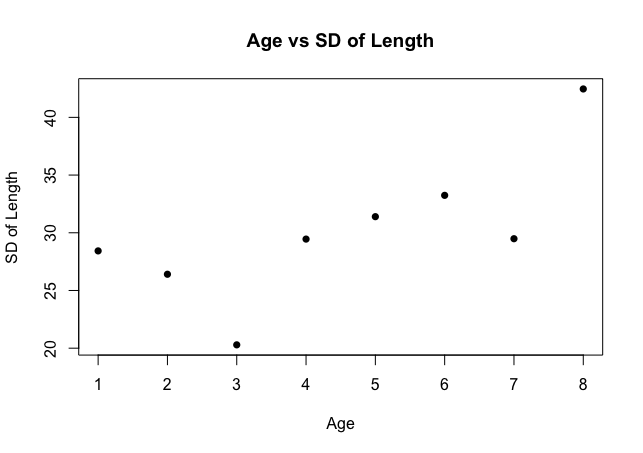
\includegraphics[scale=0.6]{1-b-1.png}

\noindent The variance of standard deviation seem to distribute around 30, except for standard deviation for age 8, which is slightly higher than others. 
\subsection*{c}
\begin{verbatim}
lm1 <- lm(wblake$Length~wblake$Scale)
plot(wblake$Scale, wblake$Length, pch=16, cex=0.5,
     xlab='Scale', ylab='Length' )
abline(lm1, col=2)

summary(lm1)
Call:
lm(formula = wblake$Length ~ wblake$Scale)

Residuals:
    Min      1Q  Median      3Q     Max 
-84.896  -9.643  -0.021  14.651  75.290 

Coefficients:
             Estimate Std. Error t value Pr(>|t|)    
(Intercept)   56.2986     2.6423   21.31   <2e-16 ***
wblake$Scale  23.3068     0.4096   56.90   <2e-16 ***
---
Signif. codes:  0 ‘***’ 0.001 ‘**’ 0.01 ‘*’ 0.05 ‘.’ 0.1 ‘ ’ 1
\end{verbatim}

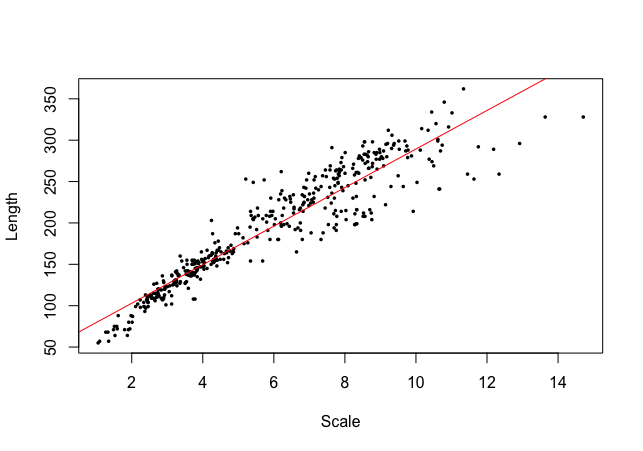
\includegraphics[scale=0.6]{1-c-1.png}

\noindent A simple linear regression line fits the data very well when scale is low, however, when scale is high, the residual increases. \\

\noindent Base on the summary of linear regression, P-value of both intercept and coefficient of scale are much less than zero, indicating that both beta zero and beta one are unlikely to be zero. 


\subsection*{d}
\begin{verbatim}
resid1 <- summary(lm1)$residual
hist(resid1, xlab='Residuals', main='Histogram of Residuals', xlim=c(-100, 100))
plot(lm(wblake$Length~wblake$Scale), which = 1, pch=16)
\end{verbatim}

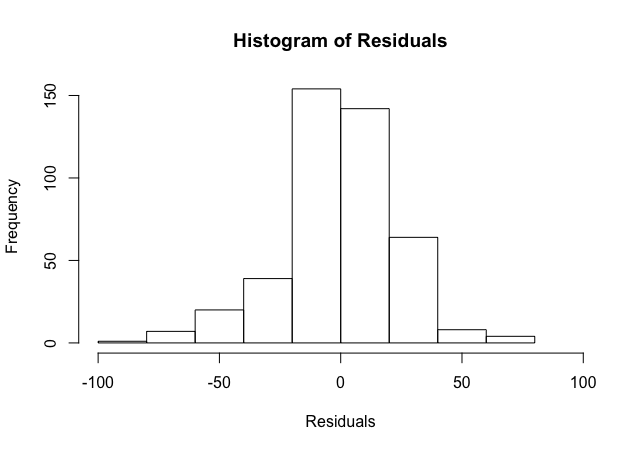
\includegraphics[scale=0.6]{1-d-1.png}

\noindent The histogram has a symmetric bell shape and centered around zero, indicating the distribution of residuals is approximately normal. The normality assumption is not violated. 

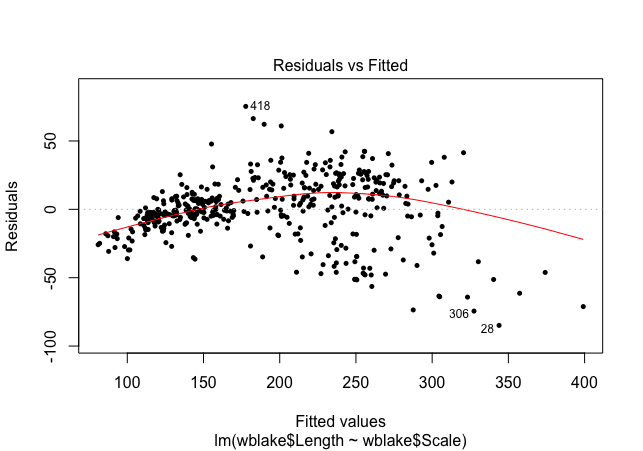
\includegraphics[scale=0.6]{1-d-2.png}

\noindent The pattern of TA plot shows that residuals randomly distributed around zero when fitted value is small. However, at the high end of fitted value, residuals tend to be farther away from zero. The relatively high curvature of line also reflects the unconstant variance within residuals. Therefore the constant variance assumption is violated. 

\subsection*{e}
\begin{verbatim}
new_pt <- data.frame(Scale=200)
fit <- lm(Length~Scale, data=wblake)
pred_200 <- predict(fit, new_pt, se.fit = T, )$fit
pred_200_CI <- predict(fit, new_pt, interval = 'confidence', level=0.95)
pred_200_PI <- predict(fit, new_pt, interval = 'prediction', level=0.95)

> pred_200
       1 
4717.665 
> pred_200_CI
       fit      lwr      upr
1 4717.665 4561.348 4873.983
> pred_200_PI
       fit     lwr      upr
1 4717.665 4554.91 4880.421
\end{verbatim}

\noindent The fitted value $\hat{y}$ for length given that scale equals 200 is 4717.665. \\

\noindent The 95 $\%$ confidence interval for fitted value is $4561.348 < \hat{y} < 4873.983$. \\

\noindent The 95 $\%$ prediction interval is $[4554.91, 4880.421]$.

\newpage
\section*{Question 2}
\subsection*{a}
\noindent Using this data set, we can analyze whether the average gdp of a country affects fertility rate. For this scenario, the predictor is gdp per person, and the response is fertility rate. 

\subsection*{b}
\begin{verbatim}
plot(x=UN1$PPgdp, y=UN1$Fertility, xlab='GDP/Person', ylab='Fertility', pch=16, cex=0.7) 
\end{verbatim}

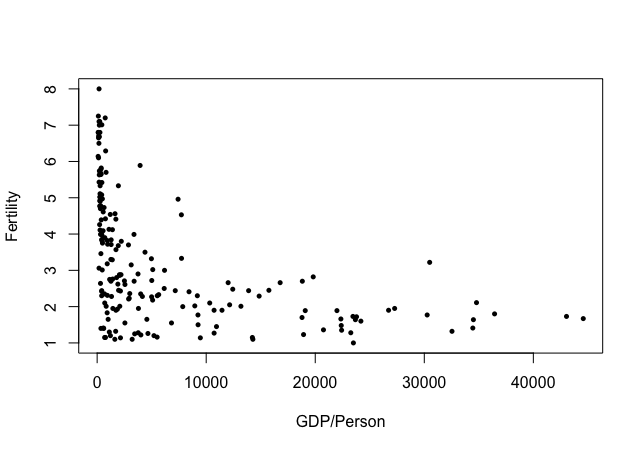
\includegraphics[scale=0.6]{2-b-1.png}

\noindent The observations at lower GDP is much more denser than high GDP. Though we may perceive that countries with high GDP generally have a low fertility rate, the unbalance in density makes linear model inappropriate here. 

\subsection*{c}
\begin{verbatim}
plot(x=log10(UN1$PPgdp), y=log10(UN1$Fertility),
     xlab='log of GDP/Person', ylab='log of Fertility', pch=16, cex=0.7) 
\end{verbatim}

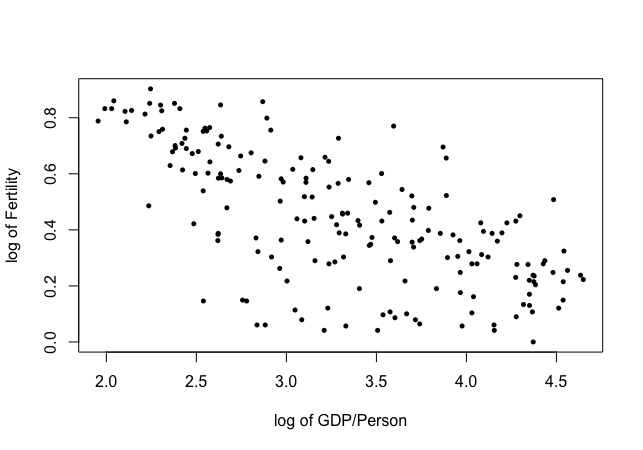
\includegraphics[scale=0.6]{2-c-1.png}

\noindent After applying log to both predictor and response, linear regression seems to fit the new data better. But the mean square error of linear model might be relatively high. 

\subsection*{d}
\begin{verbatim}
lm2 <- lm(log10(Fertility)~log10(PPgdp), data=UN1)
abline(a=lm2$coefficients[[1]], b=lm2$coefficients[[2]], col=2, lwd=2)

> summary(lm2)

Call:
lm(formula = log10(Fertility) ~ log10(PPgdp), data = UN1)

Residuals:
     Min       1Q   Median       3Q      Max 
-0.48587 -0.08148  0.03058  0.11327  0.39130 

Coefficients:
             Estimate Std. Error t value Pr(>|t|)    
(Intercept)   1.17399    0.05879   19.97   <2e-16 ***
log10(PPgdp) -0.22116    0.01737  -12.73   <2e-16 ***
---
Signif. codes:  0 ‘***’ 0.001 ‘**’ 0.01 ‘*’ 0.05 ‘.’ 0.1 ‘ ’ 1

Residual standard error: 0.1721 on 191 degrees of freedom
Multiple R-squared:  0.4591,	Adjusted R-squared:  0.4563 
F-statistic: 162.1 on 1 and 191 DF,  p-value: < 2.2e-16
\end{verbatim}

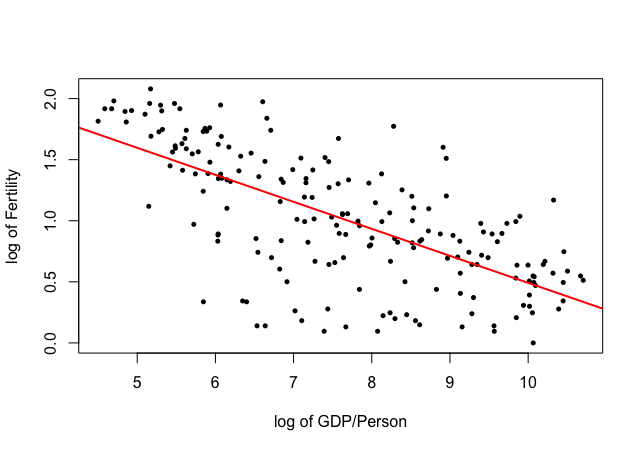
\includegraphics[scale=0.6]{2-d-1.png}

\subsection*{e}
\begin{verbatim}
hist(lm2$residuals, xlim=c(-0.5, 0.5), xlab='Residuals', main='Histogram of Residuals')

plot(lm(log(Fertility)~log(PPgdp), data=UN1), which = 1, pch=16, cex=0.7, lwd=2)
\end{verbatim}

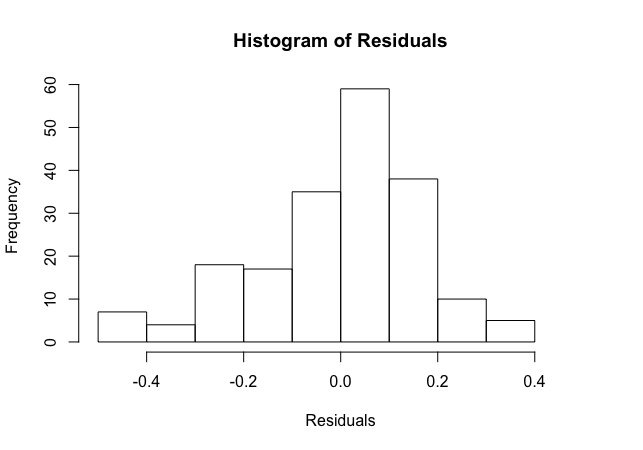
\includegraphics[scale=0.6]{2-e-1.png}

\noindent The histogram has an approximately symmetric bell shape and centered around zero, indicating the distribution of residuals is approximately normal. The normality assumption is not violated. 

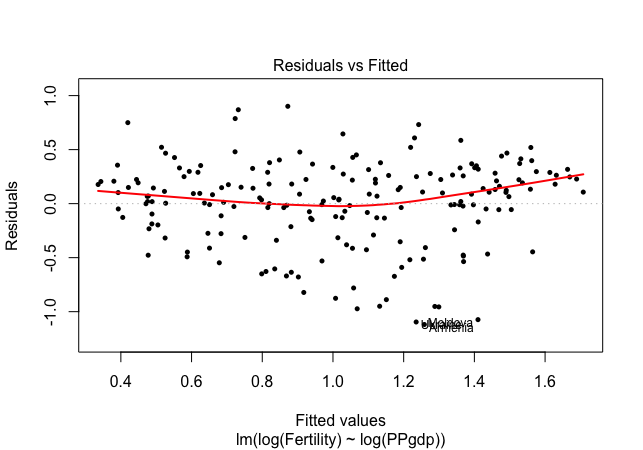
\includegraphics[scale=0.6]{2-e-2.png}

The the pattern of TA plot does not show any particular shape, implying that the correlation between residuals and fitted value is weak. The residuals scattered around zero randomly, therefore, the equal variance assumption is not violated

\subsection*{f}
\begin{verbatim}
beta1_est <- summary(lm2)$coefficient[2,1]
beta1_se <- summary(lm2)$coefficients[2,2]
t_val <- (beta1_est - 0) / beta1_se
n <- length(UN1$Fertility)

> pt(t_val, df=n-2)
[1] 1.365501e-27
> t_val
[1] -12.73366
\end{verbatim}

\noindent t-value of the slope is -12.73, the corresponding p-value is equal to $1.36 \cdot 10^{-27}$, given the null hypothesis is $\beta_1 = 0$. Since the p-value is much smaller than 0.01, we can conclude that there is strong evidence against the null hypothesis, i.e. the slope are unlikely to be zero. 

\subsection*{g}
\begin{verbatim}
confidenceEllipse(lm2,grid=TRUE,xlab="Intercept",ylab="Slope",
                  main="Rice: 99% confidence region and intervals",levels=.99, col='Skyblue')
abline(h=confint(lm2,level=.99)[2,1],lty=2,lwd=2,col="firebrick")
abline(h=confint(lm2,level=.99)[2,2],lty=2,lwd=2,col="firebrick")
abline(v=confint(lm2,level=.99)[1,1],lty=2,lwd=2,col="firebrick")
abline(v=confint(lm2,level=.99)[1,2],lty=2,lwd=2,col="firebrick")
points(1.1, -0.2, col='gray25', pch=16, cex=2)
text(1.1, -0.2, pos=4, labels='(1.1, -0.2)', cex=1)
\end{verbatim}

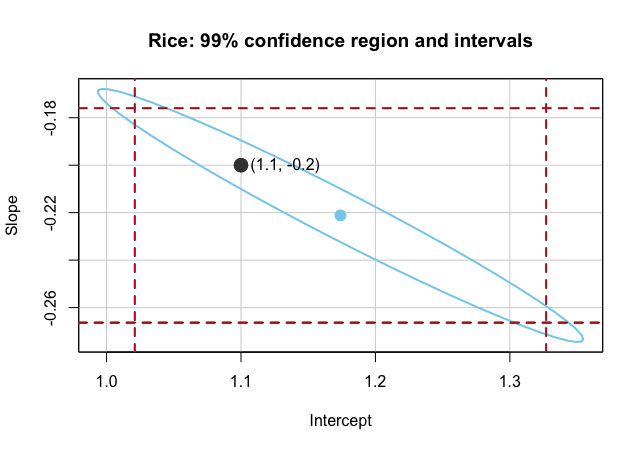
\includegraphics[scale=0.6]{2-g-1.png}

\noindent Under the confidence level of $99 \%$, I will not reject the hypothesis that $(\beta_0, \beta_1) = (1.1, -0.2)$, because the value for null hypothesis falls in the $99 \%$ confidence region. Meanwhile, both slope and intercept of the null hypothesis fall in between the marginal confidence intervals. 

\newpage
\section*{Question 3}
\subsection*{a}
\noindent We have proved in class: $\hat{\beta_1} = \sum c_i y_i$ where $c_i = \frac{x_i - \bar{x}}{SXX}$; $\hat{\beta_0} = \bar{y} - \hat{\beta_1} \bar{x}$
\begin{align*}
\hat{\beta_0} &= \bar{y} - \hat{\beta_1} \bar{x} \\
&= \frac{1}{n} \sum_i^n y_i - \sum_i^n c_i y_i \bar{x} \\
&= \sum_i^n (\frac{1}{n} - \bar{x} c_i) y_i 
\end{align*}

\noindent This shows $\hat{\beta_0}$ can be written as $\sum_i^n d_i y_i$ where $d_i =  \frac{1}{n} - \bar{x} c_i$ and $c_i = \frac{x_i - \bar{x}}{SXX}$.

\subsection*{b}
We have proved in class: $\hat{\beta_1}$ is an unbiased estimator for $\beta_1$, i.e. $E(\hat{\beta_1}| X=x) = E(\sum c_i y_i) = \beta_1$ \\

\noindent Note that $\hat{\beta_0} = \sum d_i y_i$, where $d_i =  \frac{1}{n} \bar{x} c_i$; $y_i = \beta_0 + \beta_i x_i + \epsilon_i$, $E(y_i) = \beta_0 + \beta_i x_i$
\begin{align*}
E(\hat{\beta_0} | X=x) &= E(\sum_i^n (\frac{1}{n} - \bar{x} c_i) y_i | X=x) \\
&= E(\sum \frac{1}{n} y_i | X=x) - E(\bar{x} c_i y_i | X=x) \\
&= \frac{1}{n} \sum_i^n E(y_i | X=x) - \bar{x} E(\sum_i^n c_i y_i | X=x) \\
&= \frac{1}{n} \sum_i^n (\beta_0 + \beta_i x_i) - \bar{x} \beta_1 \\
&= \beta_0 + \beta_1 \frac{1}{n} \sum_i^n x_i - \bar{x} y_i \\
&= \beta_0 + \beta_1 \bar{x} - \beta_1 \bar{x} \\
&= \beta_0
\end{align*}
\noindent This proves $\hat{\beta_0}$ is an unbiased estimator for $\beta_0$.

\subsection*{c}
\noindent Note that $\hat{\beta_0} = \sum_i^n d_i y_i$, where $d_i =  \frac{1}{n} \bar{x} c_i$ ; $Var(y_i | X = x) = Var(\epsilon_i) = \sigma^2$
\begin{align*}
Var(\hat{\beta_0} | X=x) &= Var(\sum_i^n d_i y_i | X=x) \\
&= \sum_i^n d_i^2 Var(y_i | X=x) \\
&= \sigma^2 \sum_i^n (\frac{1}{n} - \bar{x} c_i)^2 \\
&= \sigma^2 \sum_i^n (\frac{1}{n^2} - \frac{2}{n} \bar{x} c_i + \bar{x}^2 c_i^2 )
\end{align*}
\noindent Plug $c_i = \frac{x_i - \bar{x}}{SXX}$ into the equation,
\begin{align*}
Var(\hat{\beta_0} | X=x) &= \sigma^2 \sum_i^n (\frac{1}{n^2} - \frac{2}{n}  \frac{\bar{x} (x_i - \bar{x})}{SXX} + \frac{\bar{x}^2 (x_i - \bar{x})^2} {SXX^2} )\\
&= \sigma^2 (\sum_i^n \frac{1}{n^2} - \frac{2}{n}  \frac{\bar{x} \sum_i^n (x_i - \bar{x})}{SXX} + \frac{\bar{x}^2  \sum_i^n (x_i - \bar{x})^2}{SXX^2} )
\end{align*}
\noindent Note that $\sum_i^n (x_i - \bar{x}) = 0$, $\sum_i^n (x_i - \bar{x})^2 = SXX$,
\begin{align*}
Var(\hat{\beta_0} | X=x) &=\sigma^2 (\frac{1}{n} - 0 + \frac{\bar{x}^2  SXX}{SXX^2} ) \\
&= \sigma^2 (\frac{1}{n} - \frac{x^2}{SXX})
\end{align*}

\subsection*{d}
\noindent Note that $\hat{y_i} = \hat{\beta_0} + \hat{\beta_1} \bar{x}$, $\hat{\beta_0} = \bar{y} - \hat{\beta_1} \bar{x}$
\begin{align*}
\sum_i^n (y_i - \hat{y_i}) &= \sum_i^n y_i - \sum_i^n \hat{y_i} \\
&= \sum_i^n y_i - \sum_i^n \hat{\beta_0} + \hat{\beta_1} \bar{x} \\
&= \sum_i^n y_i - \sum_i^n \bar{y} - \hat{\beta_1} \bar{x} + \hat{\beta_1} \bar{x} = \sum_i^n y_i - \sum_i^n \bar{y}
\end{align*}
\noindent Note that $\sum_i^n y_i = n \bar{y}$, $\sum_i^n \bar{y} = n \bar{y}$ as well, the last equation shows $\sum_i^n (y_i - \hat{y_i}) = 0$

\newpage
\section*{4}
\subsection*{a}
\begin{align*}
\frac{d RSS}{d \beta_1} &= \sum_i^n -2 x_i (y_i - \beta_1 x_i)
\end{align*}
\noindent To minimize SSE, we want to find $\hat{\beta_1}$ such that $\frac{d RSS}{d \beta_1} = 0$.
\begin{align*}
\sum_i^n -2 x_i (y_i - \beta_1 x_i) &= 0 \\
2 \beta_1 \sum_i^n x_i^2 &=  2 \sum_i^n x_i y_i \\
\hat{\beta_1} &= \frac{\sum_i^n x_i y_i}{\sum_i^n x_i^2}
\end{align*}
\noindent This shows the least square estimation for $\beta_1$, $\hat{\beta_1} = \frac{\sum_i^n x_i y_i}{\sum_i^n x_i^2}$.

\subsection*{b}
\begin{align*}
E(\hat{\beta_1} | X=x) &= E(\frac{\sum_i^n x_i y_i}{\sum_i^n x_i^2} | X=x) \\
&= E( \frac{\sum_i^n x_i (\beta_1 x_i + \epsilon_i)}{\sum_i^n x_i^2} | X=x ) \\
&= \beta_1 E(\frac{\sum_i^n x_i^2}{\sum_i^n x_i^2 } | X=x) + E(\frac{\sum_i^n x_i \epsilon_i}{\sum_i^n x_i^2 } | X=x) \\
&= \beta_1 + \frac{1}{\sum_i^n x_i^2} \sum_i^n E(x_i \epsilon_i | X=x)
\end{align*}
\noindent Since $x_i$ and $\epsilon_i$ are independent, $E(x_i \epsilon_i) = E(x_i) E(\epsilon_i) = 0$. \\

\noindent Therefore, the last equation becomes $E(\hat{\beta_1} | X=x) = \beta_1 + 0 = \beta_1$.

\subsection*{c}
\begin{align*}
Var(\hat{\beta_1} | X=x) &= Var(\frac{\sum_i^n x_i y_i}{\sum_i^n x_i^2} | X=x) \\
&= \frac{1}{(\sum_i^n x_i^2)^2} Var(\sum_i^n x_i y_i |X=x)
\end{align*}
\begin{align*}
Var(\sum_i^n x_i y_i |X=x) &= E((\sum_i^n x_i y_i)^2 |X=x) - E(\sum_i^n x_i y_i |X=x)^2 \\
&= E(\sum_i^n \sum_j^n (x_i y_i) (x_j y_j) |X=x) - E(\sum_i^n x_i y_i |X=x) E(\sum_j^n x_j y_j |X=x) \\
&= \sum_i^n \sum_j^n [E((x_i y_i)(x_j y_j)|X=x) - E(x_i y_i |X=x)E(x_j y_j |X=x)]\\
&= \sum_i^n \sum_j^n Cov(x_i y_i, x_j y_j |X=x) \\
&= \sum_i^n \sum_j^n x_i x_jCov( y_i, y_j |X=x)
\end{align*}
\noindent Note that when $i \neq j$, $Cov(y_i, y_j) = 0$ since they are independent to each other. \\

\noindent Therefore, we get $\sum_i^n \sum_j^n x_i x_jCov( y_i, y_j |X=x) = \sum_i^n x_i^2 Var(y_i)$. 
\begin{align*}
Var(\hat{\beta_1} | X=x)  &= \frac{1}{(\sum_i^n x_i^2)^2} \sum_i^n x_i^2 Var(y_i | X=x)
\end{align*}
\noindent Note that $Var(y_i |X=x) = Var(\beta_i x_i + \epsilon_i | X=x)$ where $\beta_1$ and $x_i$ are constant. Thus $Var(y_i |X=x) = Var(\epsilon_i) = \sigma^2$.
\begin{align*}
Var(\hat{\beta_1} | X=x)  &= \frac{1}{(\sum_i^n x_i^2)^2} \sum_i^n x_i^2 \sigma^2 \\
&= \frac{\sigma^2}{\sum_i^n x_i^2}
\end{align*}


\end{document}